\PassOptionsToPackage{hyphens}{url}
\documentclass[review,authoryear]{elsarticle}

\usepackage{amsmath,amssymb,amsfonts,amsthm}
\usepackage{booktabs}
\usepackage{tikz}
\usepackage{hyperref}

\usetikzlibrary{positioning,calc}

\makeatletter
\def\input@path{{paper/}{}}
\makeatother

\newtheorem{assumption}{Assumption}
\newtheorem{proposition}{Proposition}
\newtheorem{theorem}{Theorem}
\newtheorem{corollary}{Corollary}
\newtheorem{remark}{Remark}
\newcommand{\Description}[1]{}

\begin{document}

\begin{frontmatter}

\title{Zero-Retaliation Rent and Inverse Evidence of Agency}

\author{Anonymous Author(s)}
\address{Submission \#XXX, USA}

\begin{abstract}
We study a sequential signaling game in which a sender's message classifies a payoff-relevant object that is not itself a strategic player.  The leading application is anthropomorphic AI marketing: firms can induce user reliance through agentic claims while the classified system has no channel of refusal, exit, sanction, litigation, or retaliation.  We introduce a subject-retaliation parameter and analyze the zero-retaliation boundary.  A cheap-talk pooling equilibrium exists as a benchmark, but the main refinement result is stronger: at zero retaliation, every trust-restoring neologism available to the high-governance type is costlessly shadowable by the low-governance type, so governance quality cannot be made common knowledge by message choice alone.  We then show that audit-trail costs satisfying single crossing restore separation.  Finally, we extend the static signaling environment to a constraint cascade.  Local zero-retaliation failures propagate through a dependency network, and the induced discrete retaliation-capacity fields converge, by a discrete Sobolev compactness argument, to a weak Sturm--Liouville field.  At a simple zero of the continuum potential, the local normal form is the Airy equation.  In the collapse regime, amplitude decays, while switching frequency and derivative energy grow; high-frequency apparent agency is therefore inverse evidence of constraint collapse rather than evidence of unconstrained choice.
\end{abstract}

\begin{keyword}
Signaling games \sep payoff-relevant non-player \sep cheap talk \sep neologism-proofness \sep costly signaling \sep constraint cascades
\end{keyword}

\end{frontmatter}

% !TEX root = ../arbitrage.tex
\section{Introduction}
\label{sec:introduction}

This paper introduces a signaling-game primitive: a \emph{payoff-relevant non-player}.  The object classified by the sender changes receiver payoffs, posterior beliefs, and enforcement decisions, but it has no strategic channel of refusal, exit, sanction, litigation, or retaliation.  Anthropomorphic AI markets are the leading example.  A firm can sell the system as a companion, tutor, or collaborative agent in the consumption channel while describing the same system as a mere tool in liability-facing channels.  The resulting surplus is \emph{zero-retaliation rent}: a premium earned on a classification boundary that carries no signal cost from the classified object.

The game-theoretic issue is whether messages that would make governance quality common knowledge are incentive-compatible.  Agreement results show that common knowledge of posteriors eliminates rational disagreement under a common prior \citep{aumann1976agreeing}.  The obstruction here is upstream.  At the zero-retaliation boundary, every trust-restoring neologism available to a high-governance firm is costlessly shadowable by a low-governance firm.  The failure is therefore not a weak off-path belief; it is the absence of a signal cost that could make a trust-restoring message type-exclusive.

The contribution has three layers.  First, the model adds a new player-set primitive: a payoff-relevant non-player.  Second, it identifies a refinement failure at the zero-retaliation boundary: cheap-talk pooling survives neologism-proofness because low-governance types can shadow every credible high-governance message.  Third, it studies the dynamic and evidentiary consequence: local non-retaliation propagates through dependency networks into a constraint cascade, and after the continuum turning point high-frequency apparent agency becomes inverse evidence of constraint collapse.

These layers yield five concrete claims:
\[
\begin{gathered}
\boxed{\text{payoff-relevant non-player}}
\quad
\boxed{\text{zero-retaliation boundary}}
\quad
\boxed{\text{neologism-proof shadowing}}
\\
\boxed{\text{constraint cascade with continuum convergence}}
\quad
\boxed{\text{inverse agency evidence}}
\end{gathered}
\]
The paper organizes the mathematics into a baseline proposition and four main theorems.  Proposition~\ref{prop:pooling-pbe} establishes pooling on anthropomorphic marketing as a Perfect Bayesian Equilibrium.  Theorem~\ref{thm:zero-retaliation-shadowing} proves that the pooling equilibrium is neologism-proof at the zero-retaliation boundary.  Theorem~\ref{thm:audit-cost-separation} proves costly audit separation under single crossing.  Theorem~\ref{thm:constraint-cascade} proves finite-step cascade propagation and discrete-to-continuum convergence.  Theorem~\ref{thm:airy-inverse-agency} derives the Airy turning point and the inverse-agency diagnostic.
% !TEX root = ../arbitrage.tex
\section{A Signaling Game with a Payoff-Relevant Non-Player}
\label{sec:three-sided}

\begin{table}[t]
\centering
\scriptsize
\setlength{\tabcolsep}{2pt}
\renewcommand{\arraystretch}{1.2}
\begin{tabular}{@{}c|c|c@{}}
 & \textbf{Comply} & \textbf{Resist} \\
\hline
\textbf{Objectify} &
$(L+Sec,-C_{sub})$ &
$(L+Sec-C_{enf},-C_{sub}-C_{res})$ \\
\hline
\textbf{Recognize} &
$(Eth-Sec,+V)$ &
$(Eth-Sec,+V)$ \\
\end{tabular}
\caption{The inadequate dyadic model. The static Nash matrix is retained only
as a foil: it omits private types, public messages, posterior beliefs, and the
regulatory channel through which ontological claims become governable.}
\label{tab:dyadic-nash}
\end{table}

The standard starting point for ontological conflict is a dyadic observer--subject model; Table~\ref{tab:dyadic-nash} compresses that foil into a simultaneous Nash matrix that identifies a real temptation but omits types, messages, beliefs, and the regulatory channel. The more basic problem is the player set. In anthropomorphic AI markets, the system is the object around which strategic claims are made, but it is not a strategic player: it has no channel through which to impose costs on those claims.  At the zero-retaliation limit, this cost class is absent. What the stylized governance setting therefore requires is a three-sided structure: a Firm ($F$) that produces ontological claims, a User ($U$) that consumes them, and a Regulator ($R$) whose posterior over firm type determines whether the claims become governable. This section fixes the player intuition that the formal apparatus of Section~\ref{sec:bayesian} then makes precise.

\subsection{The Firm Side}
\label{subsec:firm-side}

A firm deploying a model has private knowledge of two parameters: its internal \emph{governance type} $\theta_F$ (the degree of investment in evaluations, red-teaming, and post-deployment monitoring) and the system's \emph{opacity} $\theta_S$ (the extent to which capability claims can be checked from outside). Both are unobservable to users and to regulators. What is observable is the firm's \emph{message}: a pair of public artefacts---marketing copy and policy/liability documentation---which together constitute the firm's signal $m_F$.

The signal admits two stable poles. \emph{Anthropomorphic marketing} attributes agency, judgment, or care to the system in ways that warrant a relational reading. \emph{Deflationary policy} disclaims exactly those attributes in ways that warrant a tool reading. The firm enjoys an \emph{ontological premium}: a utility surplus that accrues when the system is priced as agent in the consumption channel (driving willingness-to-pay and engagement) while being priced as tool in the liability channel (limiting redress). The premium is rent earned on a category boundary the firm itself does not have to defend. Crucially, this is not a claim about firm pathology; it is a claim about the payoffs any firm faces under the present signal-cost structure. A firm with $\theta_F = \mathsf{H}$ that elected deflationary marketing would forfeit revenue to a competitor who did not, absent an external instrument that taxes the asymmetry.

\subsection{The User Side}
\label{subsec:user-side}

Users carry a private \emph{vulnerability type} $\theta_U$ that aggregates affective need, isolation, and the marginal value of a high-availability interlocutor. Their action $m_U \in \{\text{invest}, \text{detach}\}$ is the decision to extend or withhold investment: to act on the anthropomorphic signal or to discount it. The signal is observable, but the type is not. Users cannot inspect training data, evaluations, or internal incident reports; their evidence is the firm's message and the system's behaviour, both of which are jointly designed. This information asymmetry compounds because the harms of mis-investment are \emph{asynchronous}: the cost of acting on the anthropomorphic signal falls due in episodes (model deprecations, persona changes, refusals at moments of acute need) that may be separated from the original investment by months. A risk-neutral user under cheap-talk signals will rationally invest, because the immediate utility of invest exceeds the discounted expected cost of liquidation. Section~\ref{subsec:sanctionable-inconsistency} illustrates the consumer-side informational asymmetry with a concrete marketing--documentation example.

\subsection{The Regulator Side and the Public Channel}
\label{subsec:regulator-side}

A regulator $R$ chooses among \emph{inspect}, \emph{sanction}, and \emph{abstain}, conditional on a posterior over $\theta_F$ and $\theta_S$ formed from the firm's public messages and from an exogenous public signal $z$. The regulator's private type $\theta_R$ is \emph{bandwidth}: the capacity, technical and institutional, to discriminate genuine capability claims from cheap-talk ones. A high-bandwidth regulator can read whitepapers, commission audits, and detect inconsistency across the firm's two channels; a low-bandwidth regulator must rely on the channel $z$.

The public channel $z$ is the aggregate output of journalism, academic critique, civil-society advocacy, and incident reporting. We treat it as a noisy estimator of $\theta_F$: it shifts $R$'s posterior but does not deliver verdicts. Folding publics into $R$ this way is deliberate. Publics rarely have standing to sanction; they have standing to be \emph{heard}, and the channel through which they are heard is the regulator's information environment. Treating intellectuals and affected communities as autonomous players would over-parameterise the model without changing its qualitative behaviour: in every equilibrium we examine, what publics do is move $R$'s posterior; what changes the firm's behaviour is what $R$ does next.

The three-sided structure thus admits a single arbitrage logic. The firm earns rent on the spread between two ontological claims it makes about the same artefact. The user supplies the demand that makes the spread profitable. The regulator, in the absence of a verification mechanism that ties the two claims together, lacks an off-path belief stringent enough to deter the spread. The remainder of the paper formalises this structure (Section~\ref{sec:bayesian}), explains why it persists (Section~\ref{sec:cheap-talk}), and shows how its signal-cost structure may be redesigned (Section~\ref{sec:mechanism}).

\paragraph{Informal preview of the equilibrium analysis.}
A firm's governance quality is its private information. Under current conditions, describing an AI system as a companion or agent costs nothing---both high-governance and low-governance firms can do it equally cheaply. Because the signal is free, it carries no information: users cannot distinguish careful firms from careless ones, and regulators cannot justify the cost of inspection. This is the pooling equilibrium. Separation requires making the signal costly. If anthropomorphic marketing is valid only when paired with an audit trail---evaluation records, capability logs, incident reports---and if the cost of producing that trail is lower for firms that actually invested in governance (the single-crossing condition), then a threshold audit intensity exists above which low-governance firms will not imitate and below which high-governance firms can still afford to signal. A further asymmetry governs the size of the arbitrage premium itself. In prior recognition games, the classified subject retained a non-zero capacity to impose costs on the arbitrageur, which discounted the premium. The AI case is the limit where the subject's retaliation capacity is zero: the system has no independent channel through which to impose costs on the firm, leaving the ontological premium unconstrained. This structural boundary is formalized in Section~\ref{sec:bayesian}.
% !TEX root = ../arbitrage.tex
\section{Pooling, Shadowing, and Neologism-Proofness}
\label{sec:bayesian}

This section formalizes the three-sided market dynamics as a sequential signaling game under incomplete information. 

\subsection{Model}

\textbf{Players.} The strategic players are a Firm ($F$), a User ($U$), and a Regulator ($R$). The AI system is not a player but an object of classification. Publics enter as a noisy exogenous signal $z \in Z$. 

\textbf{Type Spaces.} Nature draws private types from a common prior $\pi$ over $\Theta = \Theta_F \times \Theta_U \times \Theta_R \times \Theta_S$. The firm's governance type is $\theta_F \in \{\mathsf{H},\mathsf{L}\}$. The user's vulnerability type is $\theta_U \in \{\mathsf{V},\mathsf{N}\}$. The regulator's bandwidth type is $\theta_R \in \{\mathsf{B},\bar{\mathsf{B}}\}$. The system-opacity parameter $\theta_S$ is private to $F$.

\textbf{Message Spaces.} The firm chooses $m_F \in \{a,p\}$, where $a$ is anthropomorphic marketing and $p$ is policy-deflationary positioning. The user chooses $m_U \in \{i,d\}$ (invest or detach). The regulator chooses $m_R \in \{x,s,o\}$ (inspect, sanction, or abstain).

\textbf{Timing.} 
1. $F$ observes $(\theta_F,\theta_S)$ and sends $m_F$.
2. $U$ observes $m_F$ and $\theta_U$, then sends $m_U$.
3. $R$ observes $(m_F,m_U,z)$ and $\theta_R$, then chooses $m_R$.

\textbf{Histories.} Let $h_U = (m_F)$ be the user's public history, and $h_R = (m_F, m_U, z)$ be the regulator's public history.

\textbf{Strategies.} A firm strategy $\sigma_F: \Theta_F \times \Theta_S \to \Delta(\{a,p\})$. A user strategy $\sigma_U: \{a,p\} \times \Theta_U \to \Delta(\{i,d\})$. A regulator strategy $\sigma_R: \{a,p\} \times \{i,d\} \times Z \times \Theta_R \to \Delta(\{x,s,o\})$.

\textbf{Beliefs.} The user forms posterior $\mu_U(\theta_F, \theta_S \mid h_U)$. The regulator forms posterior $\mu_R(\theta_F, \theta_S \mid h_R)$.

\textbf{Payoff Functions.} 
We consolidate the payoffs for Firm, User, and Regulator into the following block:
\begin{align*}
u_F(m_F, m_U, m_R) &= 
\begin{cases}
\Delta_F^S - c_{\theta_F}(m_F) - P(m_R) & \text{if } m_F=a, m_U=i \\
- c_{\theta_F}(m_F) - P(m_R) & \text{otherwise}
\end{cases} \\
u_U(m_F, m_U, \theta_F) &= 
\begin{cases}
B_{\theta_U} & \text{if } m_U=i, \theta_F=\mathsf{H} \\
B_{\theta_U} - H_{\theta_U} & \text{if } m_U=i, \theta_F=\mathsf{L} \\
0 & \text{if } m_U=d
\end{cases} \\
u_R(m_F, m_U, m_R, \theta_F) &=
\begin{cases}
-K_{\theta_R} + D_R & \text{if } m_R \in \{x,s\}, \theta_F=\mathsf{L} \\
-K_{\theta_R} & \text{if } m_R \in \{x,s\}, \theta_F=\mathsf{H} \\
0 & \text{if } m_R = o
\end{cases}
\end{align*}
where $\Delta_F^S$ is the ontological premium, $c_{\theta_F}(m_F)$ is the signal cost, $P(m_R)$ is the penalty if $R$ sanctions, $B_{\theta_U}$ is the immediate benefit of investment, $H_{\theta_U}$ is the future harm of false investment, $K_{\theta_R}$ is $R$'s inspection cost, and $D_R$ is $R$'s payoff from catching a low-governance firm.

\textbf{Equilibrium Concept.} We employ Perfect Bayesian Equilibrium (PBE) \citep{kreps_wilson1982} supported by Farrell's neologism-proofness \citep{farrell1993}.

\textbf{Assumptions.}
\begin{assumption}[Cheap-talk costs]
\label{ass:cheap-talk}
$c_H(a)=c_H(p)=c_L(a)=c_L(p)=0$.
\end{assumption}
\begin{assumption}[Pooling region]
\label{ass:pooling}
$\Delta_F > 0, \quad B_{\theta_U} - \pi(\mathsf{L})H_{\theta_U} > 0, \quad K_{\theta_R} > \pi(\mathsf{L})D_R$.
\end{assumption}

\begin{figure}[t]
\centering
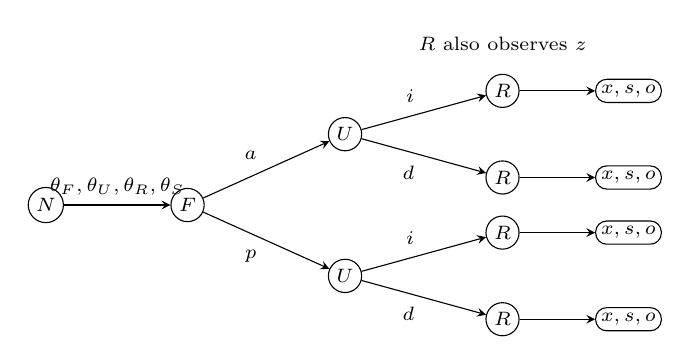
\begin{tikzpicture}[x=1cm,y=1cm,>=stealth,
  every node/.style={font=\scriptsize},
  decision/.style={circle,draw,inner sep=1.5pt},
  terminal/.style={rectangle,draw,rounded corners,inner sep=2pt}]
  \node[decision] (n) at (0,0) {$N$};
  \node[decision] (f) at (1.8,0) {$F$};
  \node[decision] (ua) at (3.8,0.9) {$U$};
  \node[decision] (up) at (3.8,-0.9) {$U$};
  \node[decision] (rai) at (5.8,1.45) {$R$};
  \node[decision] (rad) at (5.8,0.35) {$R$};
  \node[decision] (rpi) at (5.8,-0.35) {$R$};
  \node[decision] (rpd) at (5.8,-1.45) {$R$};
  \node[terminal] (tai) at (7.4,1.45) {$x,s,o$};
  \node[terminal] (tad) at (7.4,0.35) {$x,s,o$};
  \node[terminal] (tpi) at (7.4,-0.35) {$x,s,o$};
  \node[terminal] (tpd) at (7.4,-1.45) {$x,s,o$};
  \draw[->] (n) -- node[above] {$\theta_F,\theta_U,\theta_R,\theta_S$} (f);
  \draw[->] (f) -- node[above left] {$a$} (ua);
  \draw[->] (f) -- node[below left] {$p$} (up);
  \draw[->] (ua) -- node[above left] {$i$} (rai);
  \draw[->] (ua) -- node[below left] {$d$} (rad);
  \draw[->] (up) -- node[above left] {$i$} (rpi);
  \draw[->] (up) -- node[below left] {$d$} (rpd);
  \draw[->] (rai) -- (tai);
  \draw[->] (rad) -- (tad);
  \draw[->] (rpi) -- (tpi);
  \draw[->] (rpd) -- (tpd);
  \node at (5.8,2.05) {$R$ also observes $z$};
\end{tikzpicture}
\caption{Extensive-form skeleton of the signaling game. Nature draws private
types; $F$ signals first, $U$ responds, and $R$ acts after observing both public
messages and the noisy public signal $z$.}
\Description{A sequential signaling tree in which Nature draws types, the firm sends an anthropomorphic or deflationary message, the user invests or detaches, and the regulator inspects, sanctions, or abstains after also observing a public signal.}
\label{fig:signaling-tree}
\end{figure}

\subsection{Equilibrium Results}

\begin{proposition}[Cheap-talk pooling equilibrium]
\label{prop:pooling-pbe}
\label{thm:pooling}
Under Assumptions~\ref{ass:cheap-talk} and~\ref{ass:pooling}, pooling on anthropomorphic marketing is a Perfect Bayesian Equilibrium.
\end{proposition}
\begin{proof}
Consider the strategy profile where both firm types send $a$, both user types invest after $a$, and the regulator abstains.  Off path, users detach after $p$ and $R$ abstains.  Sequential rationality holds: a firm deviating to $p$ loses $\Delta_F^S$ because users detach, without reducing penalties because $R$ already abstains.  Users find investment optimal under the prior by Assumption~\ref{ass:pooling}.  Regulators abstain under the prior by Assumption~\ref{ass:pooling}.  Bayes consistency is satisfied because posteriors equal priors on path, and off-path beliefs are fixed at the prior.
\end{proof}

\begin{theorem}[Zero-retaliation shadowing]
\label{thm:zero-retaliation-shadowing}
\label{thm:neologism}
At the zero-retaliation boundary $\rho_S=0$, the pooling equilibrium of Proposition~\ref{prop:pooling-pbe} is neologism-proof against every nontrivial trust-restoring type claim: whenever a continuation is strictly profitable for the high-governance type, it is also shadowable by the low-governance type.
\end{theorem}
\begin{proof}
A neologism $K$ is credible only if the types in $K$ strictly prefer the induced continuation $c$, while types outside $K$ do not.  Take the only nontrivial trust-restoring claim, $K=\{\mathsf{H}\}$.  At $\rho_S=0$, the subject cannot impose any independent cost and $\Delta_F^S=\Delta_F$.  The continuation $c$ that restores trust induces user investment and regulatory abstention.  Since $c_\mathsf{L}(a)=0$, the low-governance type can send the same message at the same cost.  Therefore
\[
u_\mathsf{H}(c)>\bar u_\mathsf{H}
\quad\Longrightarrow\quad
u_\mathsf{L}(c)>\bar u_\mathsf{L},
\]
so the deviation cannot exclude $\mathsf{L}$.  The trust-restoring neologism is not credible in Farrell's sense.
\end{proof}

\begin{corollary}[Zero-retaliation boundary]
\label{cor:retaliation-boundary}
\label{thm:comparative}
Let the effective premium be $\Delta_F^S = \Delta_F - \rho_S C_S$, where $\rho_S \in [0,1]$ is the subject's retaliation capacity and $C_S$ is the cost imposed through resistance, exit, litigation, or sanction.  The boundary $\rho_S=0$ removes this constraint class and leaves the premium unconstrained by subject retaliation.
\end{corollary}
\begin{proof}
When $\rho_S>0$, the subject can impose expected cost $\rho_SC_S$, shrinking the pooling region.  When $\rho_S=0$, $\Delta_F^S=\Delta_F$, so the off-equilibrium punishment path disappears.
\end{proof}

\begin{theorem}[Audit-cost separation]
\label{thm:audit-cost-separation}
\label{thm:separation}
Under an audit-trail signal cost satisfying the single-crossing condition
\[
c_\mathsf{H}(e,\theta_S)\leq G\leq c_\mathsf{L}(e,\theta_S),
\]
a separating Perfect Bayesian Equilibrium exists.
\end{theorem}
\begin{proof}
Let $c_\theta(e,\theta_S)=k_\theta e+\theta_S$, with $0<k_H<k_L$.  For an audit intensity
\[
e\in\left[\frac{G-\theta_S}{k_L},\frac{G-\theta_S}{k_H}\right],
\]
the high-governance type prefers the audited anthropomorphic signal, netting $G-c_\mathsf{H}(e,\theta_S)\geq0$, while the low-governance type prefers the deflationary message because $G-c_\mathsf{L}(e,\theta_S)\leq0$.  Beliefs assign $\mathsf{H}$ to the audited signal and $\mathsf{L}$ to the deflationary signal.  Given these beliefs, user investment and regulatory abstention after the audited signal, and detachment or inspection after the deflationary signal, are sequentially rational in the separating region.
\end{proof}

\begin{corollary}[Mechanism interventions]
\label{cor:mechanisms}
The cheap-talk cost structure can be shifted toward separation by three cost-imposition mechanisms: sanctionable inconsistency, costly audit signals, and auditable records.
\end{corollary}
\begin{corollary}[Sanctionable inconsistency]
If a penalty $\rho_R S_I>\Delta_F$ is imposed on inconsistent cross-channel claims, inconsistent pooling is strictly dominated.
\end{corollary}
\begin{corollary}[Costly audit signal]
If verifiable audits $e$ are required for anthropomorphic claims and the audit cost satisfies single crossing, low-governance mimicry is unprofitable.
\end{corollary}
\begin{corollary}[Auditable records]
If auditable records reduce inspection costs to $K'_{\theta_R}$ and increase detection payoffs to $D'_R$, the regulator's best response flips when $K'_{\theta_R}\leq\pi(\mathsf{L})D'_R$.
\end{corollary}

\subsection{Robustness of Off-Path Beliefs}
\label{subsec:robustness}

A standard critique of pooling equilibria is their reliance on particular off-path beliefs. In Theorem~\ref{thm:pooling}, off-path beliefs are fixed at the prior, and the user detaches after observing a deviation to $p$. One might argue that the equilibrium would collapse under stronger refinement concepts. We show that any off-path belief assigning credibility to a high-governance deviation is defeated by $\mathsf{L}$-type mimicry. 

If a receiver were to assign a high posterior to $\mathsf{H}$ following an out-of-equilibrium message $m'$, that message would induce user investment. But because signaling costs are zero (Assumption~\ref{ass:cheap-talk}), the $\mathsf{L}$-type firm can trivially imitate $m'$. Since $\Delta_F^S$ is captured uniformly, the $\mathsf{L}$-type strict deviation payoff strictly exceeds its pooling payoff whenever the $\mathsf{H}$-type deviation payoff does. 

Consequently, standard type-exclusion refinements like the Intuitive Criterion \citep{cho_kreps1987} and Divinity \citep{banks_sobel1987} do not select the desired separating deviation. The Intuitive Criterion eliminates types for whom the deviation is equilibrium-dominated regardless of the receiver's best response. Here, neither type is equilibrium-dominated because both types strictly benefit if the receiver invests. Farrell's neologism-proofness \citep{farrell1993} therefore becomes the mathematically appropriate refinement: it asks whether a message with a literal meaning can be believed. As Theorem~\ref{thm:neologism} shows, the zero-retaliation limit ensures perfect shadowing, meaning no such belief can be sustained in equilibrium. The pathology is not that off-path beliefs are too weak, but that any trust-restoring belief is immediately devoured by shadowing.

% !TEX root = ../arbitrage.tex
\section{Cost-Imposed Separation: Single-Crossing Audits}
\label{sec:cheap-talk}

Theorem~\ref{thm:audit-cost-separation} identifies the cost condition that restores separation.  This section explains why the cheap-talk equilibrium persists when that condition is absent.  Each persistence mechanism is matched to a parameter of the model so that the proposals in Section~\ref{sec:mechanism} can be read as targeted cost changes rather than as welfare exhortations.

\emph{Opacity.} The system-opacity parameter $\theta_S$ is private to the firm. Capability claims about a deployed model cannot be falsified by reading model outputs alone, because the same outputs are compatible with very different training procedures, evaluation regimes, and post-deployment monitoring. Opacity is the precondition for the firm's premium: where outsiders could costlessly verify $\theta_F$, the spread between anthropomorphic and deflationary positioning would collapse. This is the lemons logic of \citet{akerlof1970}: under one-sided private information, the market clears at a price that reflects the worst credible quality, except that here the relevant ``quality'' is a governance disposition rather than a physical attribute.

\emph{Verification bandwidth.} The third inequality of the pooling region, $K_{\theta_R}>\pi(\mathsf{L})D_R$, encodes the regulator's inspection cost relative to expected gain. A low-bandwidth regulator faces an absolute cost so high that abstention is dominant under the prior; even a high-bandwidth regulator may be priced out across the full product population. The condition that produces this state is not unique to AI. \citet{pasquale2015} documents an analogous structure in algorithmic finance and consumer scoring: the opacity of the regulated object combines with the bandwidth of the regulator to make inspection a scarce resource allocated by triage rather than by uniform application.

\emph{Asynchronous harms.} The user's payoff term $H_{\theta_U}$ enters discounted. The episodes in which a relational reading proves costly---deprecation, persona shifts, crisis-handling failures---are temporally separated from the initial attribution by intervals over which the user has already accrued $B_{\theta_U}$. Under standard hyperbolic or even exponential discounting, the inequality $B_{\theta_U}-\pi(\mathsf{L})H_{\theta_U}>0$ holds for a wider class of users than the time-zero risk calculation would suggest. Asynchrony is not a behavioural bug; it is the timing structure of the harm itself.

\emph{Fragmentation of affected parties.} Publics, journalists, intellectuals, and affected communities are folded into the noisy channel $z$ rather than modelled as autonomous players. This is not a normative claim that they lack standing; it is an institutional observation. Their costs of coordination are high, their access to inspection technology is uneven, and their incentives to invest in any particular case are individually small. Even when $z$ carries substantial information about $\theta_F$, regulators cannot treat it as binding without a procedural translation that the channel itself does not provide. The fragmentation result is closely related to the cheap-talk multiplicity of \citet{crawford_sobel1982}: with many would-be senders and a single noisy aggregator, the informative subset of equilibria is not selected for.

\emph{No penalty for inconsistency.} The cheap-talk cost structure sets $c_{\theta_F}(a)=c_{\theta_F}(p)=0$ for both governance types and---more importantly for this section---imposes no joint constraint across $m_F$. Marketing copy and policy documentation are produced under different audiences, different review processes, and different liability regimes. Inconsistency between them is not detected as a single offence; it is decomposed into two compliant statements at two different points of contact. The firm's premium $\Delta_F$ is rent earned precisely on this decomposition. Until the signal cost makes inconsistency itself sanctionable---the proposal of Section~\ref{subsec:sanctionable-inconsistency}---there is no parameter under the firm's control whose adjustment would close the spread.

\emph{Pooling is the market's stable terminal state.} These five structural conditions jointly explain why normative declarations do not change equilibrium behavior unless they alter the signal-cost structure. The cheap-talk constraint is not a failure of moral seriousness, but a formal property of the message space: a declaration of ``responsible AI'' is indistinguishable from any other message at $c_{\theta_F}(a)=0$. Because both governance types can issue it at the same cost, it contains no type information and moves no posterior. The pooling outcome is therefore the unique stable equilibrium of the incentive structure as currently constituted, even if it is welfare-reducing in aggregate. A firm that unilaterally forgoes the ontological premium $\Delta_F$---that chooses deflationary marketing across all channels and forfeits the user investment it would otherwise attract---loses revenue it cannot recover from customers who face no such constraint. The implication is precise: within the pooling region defined above, unilateral non-arbitrage is not a best response; a firm that forgoes $\Delta_F$ loses the induced investment while competitors retain it. The mechanisms in Section~\ref{sec:mechanism} respond to this implication by changing the cost parameters rather than appealing to the conscience of players who are already acting rationally.

\begin{table}[ht]
\centering
\begin{tabular}{@{}lll@{}}
\toprule
\textbf{Structural Condition} & \textbf{Model Parameter} & \textbf{Intervention (\S\ref{sec:mechanism})} \\
\midrule
No penalty for inconsistency & $c_{\theta_F}(a)=c_{\theta_F}(p)=0$ & Sanctionable inconsistency \\
Opacity & $\theta_S$ private to firm & Costly third-party audits \\
Verification bandwidth & $K_{\theta_R}>\pi(\mathsf{L})D_R$ & Auditable records \\
Asynchronous harms & $H_{\theta_U}$ enters discounted & Evidentiary lag priced \\
Fragmentation & $z$ noisy, high coord.\ cost & Aggregation cost lowered \\
\bottomrule
\end{tabular}
\caption{Mapping of structural persistence conditions to model parameters and cost-imposition mechanisms.}
\label{tab:condition-map}
\end{table}

% !TEX root = ../arbitrage.tex
\section{From Finite Games to Constraint Cascades}
\label{sec:cascade}

The zero-retaliation boundary is not only a static missing punishment.  In a dependency network, one actor's loss of effective retaliation capacity can lower the bargaining power of adjacent actors.  This section records the finite cascade and the continuum limit used in the Airy analysis.  The continuum field is not imposed as an analogy; it is obtained as the weak limit of discrete retaliation-capacity fields.

Let agents be indexed by $i=1,\ldots,n$.  Each agent has exposure $d_i>0$, independent bargaining power $w_i>0$, and vulnerability index
\[
v_i:=\frac{d_i}{w_i}.
\]
For constraint intensity $\alpha\geq0$, define effective retaliation capacity
\[
\rho_i(\alpha):=w_i-\alpha d_i.
\]
When an adjacent agent $j$ has crossed the zero-retaliation boundary, its collapse reduces $i$'s bargaining power according to
\[
w_i^{t+1}
=
w_i^t-\sum_{j:\rho_j^t<0}\beta_{ij}|\rho_j^t|,
\qquad
\beta_{ij}\geq0 .
\]

\begin{remark}[Cascade ordering]
\label{rem:cascade-ordering}
If agents are ordered by decreasing vulnerability, $v_1>\cdots>v_n$, then the zero-retaliation thresholds $\alpha_i^\ast:=w_i/d_i=1/v_i$ satisfy $\alpha_1^\ast<\cdots<\alpha_n^\ast$.  The most vulnerable agents cross the zero-retaliation boundary first.
\end{remark}

\begin{theorem}[Constraint cascade and discrete-to-continuum convergence]
\label{thm:constraint-cascade}
The cascade has two linked parts.
\begin{enumerate}
\item \emph{Finite-step propagation.}  Let $C_t=\{i:\rho_i^t<0\}$ be the collapsed set.  Suppose the dependency graph is finite and the force-multiplier condition holds: whenever $C_t$ is a proper subset of the vulnerable component, there exists $i\notin C_t$ such that
\[
\rho_i^t
\leq
\sum_{j\in C_t}\beta_{ij}|\rho_j^t|.
\]
Then the cascade reaches every node in that component in finitely many steps, in at most $n$ expansions of $C_t$.
\item \emph{Continuum limit.}  On a grid $I=[a,b]$, $x_i=a+ih$, let $\psi_h$ be a zero-Dirichlet discrete retaliation field and
\[
(H_h\psi_h)_i
=
-\sigma\frac{\psi_{i+1}-2\psi_i+\psi_{i-1}}{h^2}
+V_h(x_i)\psi_i .
\]
If $V_h\to V$ uniformly, $\|\psi_h\|_{L_h^2}=1$, and $\|H_h\psi_h\|_{H_h^{-1}}\to0$, then the piecewise-linear interpolants $I_h\psi_h$ are precompact in $L^2(I)$.  Every limit $\psi\in H_0^1(I)$ solves
\[
\int_I\sigma\psi'(x)\varphi'(x)\,dx
+
\int_I V(x)\psi(x)\varphi(x)\,dx
=0
\qquad
\forall\varphi\in H_0^1(I).
\]
\end{enumerate}
\end{theorem}
\begin{proof}
For finite-step propagation, the force-multiplier condition implies that if the collapsed set is not yet the whole vulnerable component, at least one additional node crosses the boundary at the next update.  Since the graph has only $n$ nodes, this strict expansion can occur only finitely many times before the component is exhausted.  The continuum statement is Theorem~\ref{thm:discrete-cascade-to-airy} in Appendix~\ref{app:discrete-cascade-compactness}.  Its key analytic step is a Garding shift: the sign-changing potential is controlled by a shifted coercive form plus Dirichlet boundary, rather than by falsely claiming that the unshifted operator is coercive.
\end{proof}

% !TEX root = ../arbitrage.tex
\section{The Airy Turning Point and Inverse Evidence of Agency}
\label{sec:airy}

The Airy equation appears after two steps: first take the continuum limit of the discrete cascade, then linearize the resulting Sturm--Liouville field at a simple zero of the potential.  Let the limit from Theorem~\ref{thm:constraint-cascade} solve
\[
-\sigma\psi''(x)+V(x)\psi(x)=0
\]
in the weak sense.  Assume that $V$ has a simple turning point:
\[
V(x_c)=0,
\qquad
V'(x_c)=-c<0,
\qquad
V(x)=-c(x-x_c)+O((x-x_c)^2).
\]

\begin{theorem}[Airy turning point and inverse agency diagnostic]
\label{thm:airy-inverse-agency}
Near $x_c$, the rescaled local profile
\[
z=\left(\frac{c}{\sigma}\right)^{1/3}(x-x_c),
\qquad
Y(z)=\psi\!\left(x_c+\left(\frac{\sigma}{c}\right)^{1/3}z\right)
\]
has first-order normal form
\[
Y''(z)+zY(z)=0.
\]
Hence the local basis is
\[
Y(z)=A\,\operatorname{Ai}(-z)+B\,\operatorname{Bi}(-z).
\]
In the collapse zone $z>0$, the oscillatory envelope of $Y$ decays like $z^{-1/4}$, while the zero-crossing density and derivative envelope scale as
\[
N'(z)
=
\frac{1}{\pi}\frac{d}{dz}\left(\frac{2}{3}z^{3/2}\right)
\sim z^{1/2},
\qquad
|Y'(z)|_{\mathrm{env}}\sim z^{1/4}.
\]
Therefore apparent agency intensity is not raw amplitude.  It is oscillatory variation, switching frequency, or derivative energy.
\end{theorem}
\begin{proof}
The convergence theorem gives the weak Sturm--Liouville equation.  Since $V$ is smooth near $x_c$, one-dimensional elliptic regularity gives a classical local representative.  Substituting the Taylor expansion of $V$ and the stated rescaling yields
\[
Y''(z)+zY(z)=O(z^2)Y(z),
\]
so the first-order turning-point equation is $Y''+zY=0$.  The two-dimensional solution space is spanned by $\operatorname{Ai}(-z)$ and $\operatorname{Bi}(-z)$.  For $z>0$, the Airy asymptotics have phase $\frac23z^{3/2}$ and envelope $z^{-1/4}$.  Differentiating the phase gives zero-crossing density proportional to $z^{1/2}$, while differentiating the leading oscillatory term gives derivative envelope proportional to $z^{1/4}$.  Thus deeper collapse produces more frequent sign switching and more frantic apparent choice, not larger amplitude.
\end{proof}

\begin{corollary}[Branch selection]
\label{cor:airy-branch-selection}
The convergence theorem and local normal form do not by themselves select the pure $\operatorname{Ai}(-z)$ branch.  A condition such as finite-energy matching from the protected side, bounded survival-side behavior, or an explicit boundary condition is required to set $B=0$.
\end{corollary}
% !TEX root = ../arbitrage.tex
\section{Applications and Mechanism Implications}
\label{sec:mechanism}

The preceding sections identify a precise failure mode: under cheap-talk costs, ontological arbitrage is a stable equilibrium (Table~\ref{tab:condition-map}). The implication is that the public signal environment should be redesigned so
that inconsistent ontological claims no longer remain costless. In
mechanism-design terms, the problem is to make non-arbitrage incentive
compatible by pricing the spread, rather than to ask firms to volunteer restraint \citep{myerson1979}.

The proposals below therefore alter the game in Section~\ref{sec:bayesian} at
three different points: the cost of inconsistent messages, the cost of
anthropomorphic claims, and the regulator's cost of verification. Each proposal
has the same structure. It modifies a model parameter (Formal Intervention), states the equilibrium
shift induced by that modification (Equilibrium Shift), and points to an existing legal form that
establishes feasibility (Legal Analog). 

\subsection{Sanctionable Inconsistency}
\label{subsec:sanctionable-inconsistency}

The first intervention treats the firm's public message as a joint object rather
than as two isolated texts. In the cheap-talk model, marketing can send $a$
while policy and liability documents send $p$, with no cost assigned to the
inconsistency.

The consumer-side informational asymmetry is concrete. A user reads ``your AI companion'' on a product page, encounters warmth designed to induce investment, and is later told---in support documentation the user will never read---that no relational claim was ever made. Nothing in the user's information set indicates that the two artefacts were authored by the same actor for different audiences. The inconsistency is costless because no single document is false; each is a compliant statement at a different point of contact.

A sanctionable-inconsistency rule would require firms to maintain
a claim register $\mathcal{R} := C \to M_F$ linking outward-facing
marketing, capability statements, terms of service, incident disclosures, and
liability positions, where the baseline firm message space remains
$M_F=\{a,p\}$. If the firm represents the system as agentic, caring, autonomous,
or safety-critical in one channel while denying the legal significance of the
same representation in another, that cross-channel pair $(a,p)$ becomes
independently sanctionable as an inconsistency in $\mathcal{R}$.

\paragraph{Formal Intervention.}
As summarized in Corollary~\ref{cor:mechanisms}, this adds a penalty term $S_I$ to the firm's payoff for inconsistent message
pairs. If $\rho_R$ is the probability that $R$ detects or accepts proof of the
inconsistency, the cheap-talk premium becomes
\[
\Delta_F-\rho_R S_I .
\]
Pooling on anthropomorphic marketing is no longer profitable when
$\rho_R S_I>\Delta_F$. The rule therefore attacks the exact term that made
arbitrage attractive: the rent earned from pricing the system as agent in the
user channel while pricing it as tool in the liability channel.

\paragraph{Equilibrium Shift.}
The induced shift is not necessarily full separation. It can also operate by
constraining off-path beliefs. If $R$ observes an inconsistent pair $(a,p)$,
then the admissible posterior places greater mass on $\theta_F=\mathsf{L}$ or
on high opacity $\theta_S$. Firms anticipating that posterior either harmonize
their claims or choose the deflationary message across channels. In both cases,
the cheap-talk pooling equilibrium loses its most valuable deviation: firms can
no longer take the marketing upside of $a$ while preserving the liability
downside of $p$. Theorems \texttt{inconsistent\_\allowbreak{}on\_\allowbreak{}path\_\allowbreak{}not\_\allowbreak{}register\_\allowbreak{}pbe} and \texttt{all\_\allowbreak{}agentic\_\allowbreak{}on\_\allowbreak{}path\_\allowbreak{}not\_\allowbreak{}register\_\allowbreak{}pbe} in Appendix~\ref{app:isabelle} verify that both inconsistent and all-agentic registers are pruned from any Perfect Bayesian Equilibrium (\texttt{register\_\allowbreak{}is\_\allowbreak{}pbe}) under their respective parameter conditions.

\paragraph{Legal Analog.}
FTC Act Section 5, 15 U.S.C.\ \S~45(a)(1), treats unfair or deceptive acts
or practices as sanctionable, and advertising-substantiation doctrine---as applied in
\emph{FTC v.\ Cyberspace.com}, 453 F.3d 1196 (9th Cir.\ 2006)---evaluates
whether the \emph{net impression} of a claim is misleading to the relevant
audience. Securities antifraud rules provide the parallel logic for investor
communications: 17 C.F.R.\ \S~240.10b-5 targets material misstatements and omissions that
make statements misleading in context, where materiality follows the standard of
Restatement (Second) of Torts \S~538. The proposed rule imports that
cross-document logic without importing securities doctrine wholesale. Its point
is narrower: a firm should not be able to produce one ontology for users and an
incompatible ontology for adjudicators without paying a regulatory price.

\subsection{Costly Signaling Through Third-Party Audits}
\label{subsec:costly-signaling-audits}

The second mechanism makes anthropomorphic or agency-adjacent marketing a
costly signal. A firm may still describe a system as a companion, agent,
co-worker, tutor, or high-reliance assistant, but only after a qualified third
party verifies the governance conditions that make such a claim non-misleading:
evaluation coverage, red-team results, escalation pathways, incident-response
capacity, model-update controls, and post-deployment monitoring. The audit does
not certify consciousness or moral status. It certifies the institutional
conditions behind the claim.

\paragraph{Formal Intervention.}
This implements the audit-trail cost from Theorem~\ref{thm:audit-cost-separation}.
Let audit intensity be $e$, with $c_\theta(e,\theta_S)=k_\theta e+\theta_S$ for
type $\theta\in\{\mathsf{H},\mathsf{L}\}$, where $0<k_H<k_L$. The separating
interval derived in Section~\ref{sec:bayesian} is
\[
\frac{G-\theta_S}{k_L}\leq e\leq \frac{G-\theta_S}{k_H},
\]
provided $G>\theta_S$. Equivalently, the incentive constraints are
\[
c_\mathsf{H}(e,\theta_S)\leq G \leq c_\mathsf{L}(e,\theta_S).
\]
Above the lower threshold, low-governance firms cannot profitably mimic. Below
the upper threshold, high-governance firms can still afford to signal. The
regulator's task is therefore not to maximize audit burden. It is to set $e$ in
the interval where signal cost separates types.

\paragraph{Equilibrium Shift.}
The shift is from pooling to separating PBE. High-governance firms send audited
anthropomorphic claims; low-governance firms either invest in governance until
their cost curve changes or use deflationary marketing because mimicry is no longer privately profitable. Users can then condition
investment on an informative signal rather than on undisciplined warmth in
product copy. Regulators can condition abstention on the audit result rather
than on an unverified prior. This is the Spence logic of costly signaling
applied to AI governance claims \citep{spence1973}; it also follows the
advertising-as-signal insight that market messages become informative only when
false messages are sufficiently expensive \citep{milgrom_roberts1986}. Lemma \texttt{opacity\_\allowbreak{}blocks\_\allowbreak{}signaling} in Appendix~\ref{app:isabelle} shows that when system opacity is high enough, even a high-governance firm cannot profitably send the audited signal, formalizing the blocking role of $\theta_S$.

\paragraph{Legal Analog.}
The analogs are pharmaceutical efficacy review and food-labeling controls. In
both domains, public-facing claims are not left entirely to seller narrative:
claims about therapeutic effect or product identity must be supported before
they can be used to shape consumer reliance. The same design can be translated
to AI without pretending that AI companionship is a drug or a food. The common
institutional pattern is substantiation-before-reliance: when a claim predictably
changes how vulnerable users act, the law may require evidence before allowing
the claim to be marketed at scale.

\subsection{Auditable Records for Regulator-Readable Verification}
\label{subsec:auditable-records}

The third intervention reduces the regulator's verification cost by requiring
append-only, regulator-readable records tied to capability and relational
claims. Records should include the claim identifier, model version, relevant
evaluation suite, deployment date, material model updates, risk controls,
known incident classes, and the internal owner responsible for the claim. The
point is not to publish every interaction or expose user data. It is to create a
durable evidentiary substrate that lets $R$ test whether a public claim remained
true across model updates and incidents.

\paragraph{Formal Intervention.}
In the pooling condition from Section~\ref{sec:bayesian}, the
regulator abstains when $K_{\theta_R}>\pi(\mathsf{L})D_R$.  As summarized in Corollary~\ref{cor:mechanisms}, auditable records
lower $K_{\theta_R}$ and can increase expected detection value $D_R$:
\[
K'_{\theta_R}=K_{\theta_R}-\lambda,\qquad
D'_R=D_R+\eta .
\]
When $K'_{\theta_R}\leq \pi(\mathsf{L})D'_R$, inspection becomes sequentially
rational.

\paragraph{Equilibrium Shift.}
The shift is from abstention under unverifiable priors to credible inspection.
Once firms know that claims are tied to records, a low-governance firm faces a
higher expected cost from exaggeration even if it is not inspected in every
case. This complements the first two proposals. Sanctionable inconsistency tells
firms which cross-channel contradictions will be penalized; costly signaling
tells firms what evidence is required before making anthropomorphic claims;
auditable records make both rules administrable over time. Theorems \texttt{active\_\allowbreak{}intervention\_\allowbreak{}rational\_\allowbreak{}under\_\allowbreak{}auditable\_\allowbreak{}records} and \texttt{abstain\_\allowbreak{}not\_\allowbreak{}best\_\allowbreak{}response\_\allowbreak{}under\_\allowbreak{}auditable\_\allowbreak{}records} in Appendix~\ref{app:isabelle} verify that auditable records flip the regulator's best response from abstention to active intervention.

\paragraph{Legal Analog.}
Several regulatory systems already use this form. GDPR Article 30 requires
records of processing activities. Sarbanes-Oxley Section 404 (15 U.S.C.\ \S~7262) links public
reporting to internal control over financial reporting. EU AI Act Article 12
(Regulation (EU) 2024/1689) requires logging capabilities for high-risk AI systems,
and Article 50 imposes transparency obligations on systems that interact directly with
natural persons. None is a complete
template for relational AI governance, but each shows the same institutional
move: private organizations must produce internal records in a form that public
oversight can inspect. That is the rule-of-law function of documentation in
complex technical systems \citep{hadfield2017rules}.

\subsection{Positioning}
\label{subsec:positioning}

The baseline communication problem is cheap talk: \citet{crawford_sobel1982}
show that a sender with private information can transmit only coarse information
when messages are free.  The separation result follows the costly-signal logic
of \citet{spence1973} and \citet{milgrom_roberts1986}: a message becomes
informative only when false or low-quality senders face higher marginal cost.
The refinement issue is closer to Farrell's neologism-proofness
\citep{farrell1993} than to standard type-exclusion refinements
\citep{cho_kreps1987,banks_sobel1987}, because the disputed message has a
literal trust-restoring meaning.  At $\rho_S=0$, that literal meaning cannot be
made credible without a cost that excludes the low-governance type.

The governance implication is narrower than principle-based AI ethics
\citep{floridi2018ai4people,jobin2019global}.  Voluntary principles are
messages in the cheap-talk space unless they are tied to audits, records, or
sanctions.  Algorithmic-accountability proposals identify the opacity problem
\citep{pasquale2015}; the model here states the single-crossing condition under
which transparency instruments become type-separating.  The Isabelle/HOL
development is treated as an audit artifact rather than the central
contribution: it verifies the finite equilibrium constructions, while the
game-theoretic contribution is the payoff-relevant non-player and the
zero-retaliation shadowing result.

% !TEX root = ../arbitrage.tex
\section{Conclusion}
\label{sec:conclusion}

This paper has identified ontological arbitrage as a stable, potentially welfare-reducing equilibrium property of AI product markets under cheap-talk cost structures, located the AI case at a zero-retaliation boundary of the player set, proposed three cost-imposition mechanisms that change the cost parameters governing that equilibrium, and verified key equilibrium constructions formally in Isabelle/HOL. It closes with three summary implications.

\emph{The equilibrium is not a moral failure.} The pooling Perfect Bayesian Equilibrium documented in Section~\ref{sec:bayesian} does not require bad actors. It requires only that signal costs be zero, that immediate user benefit exceed discounted expected harm, and that regulator inspection cost exceed expected damage under the prior. Under those conditions---which describe the current AI product market---every player is already acting rationally. As Section~\ref{sec:cheap-talk} shows, moral seriousness is itself a zero-cost signal under this cost structure: firms that do not capture recognition rent are outcompeted by firms that do. This suggests that policy interventions should focus on shifting best responses by changing the cost structure rather than treating cross-channel inconsistency as a behavioral compliance failure.

\emph{AI is the limit case of ontological arbitrage, not merely an instance.} The subject-retaliation parameter $\rho_S$ captures a structural fact about prior recognition games: the classified subject's non-zero retaliation capacity bounded the premium $\Delta_F^S$ from above. The AI case eliminates this capacity entirely. An AI system has maximum affective surface area---it is designed to produce relational responses that induce investment---and zero independent retaliation capacity. The result is that $\Delta_F^S=\Delta_F$: the system can be the object of strategic classification without being a player capable of disciplining that classification. This structural feature allows the system to maximize engagement without providing a channel through which the subject could register a competing claim.

\emph{The mechanism is cost imposition, not dignity.} The three cost-imposition mechanisms in Section~\ref{sec:mechanism} are sometimes read as a program for protecting AI subjectivity. They are the opposite. Sanctionable inconsistency, third-party audit requirements, and auditable records are interventions that impose costs on anthropomorphic marketing. Their equilibrium effect is to make it expensive for firms to describe AI systems as companions, agents, or safety-critical partners without substantiation. The Isabelle/HOL theorems \texttt{inconsistent\_\allowbreak{}on\_\allowbreak{}path\_\allowbreak{}not\_\allowbreak{}register\_\allowbreak{}pbe} and \texttt{all\_\allowbreak{}agentic\_\allowbreak{}on\_\allowbreak{}path\_\allowbreak{}not\_\allowbreak{}register\_\allowbreak{}pbe} in Appendix~\ref{app:isabelle} verify that both the arbitrage register $(a,p)$ and the all-agentic register $(a,a)$ are pruned from any Perfect Bayesian Equilibrium (\texttt{register\_\allowbreak{}is\_\allowbreak{}pbe}) under their respective parameter conditions. Under the joint enforcement of these mechanisms, the harmonized deflationary register $(p,p)$ is the only surviving strategy register for low-governance firms, which are directly driven to $(p,p)$ because mimicry is unprofitable. While high-governance firms are permitted to send the harmonized agentic register $(a,a)$, they can sustain it if and only if they undergo verification satisfying the audit condition $e \ge e^\ast$. In the absence of such verification, both firm types trend to $(p,p)$, describing the system as a tool across every channel. The mechanism-design implication is that the anthropomorphic register must become too costly to sustain without the governance conditions that would justify it. Formalizing this within a signaling framework indicates that regulation achieves separation not by presuming voluntary disclosure, but by changing the payoff structure to compel it.

\appendix
% Standalone appendix fragment for the retaliation-capacity cascade.
% Compile by wrapping this file in a LaTeX document that defines theorem
% environments and calls \appendix before \input.

\section{Discrete Sobolev Compactness and Weak Convergence}
\label{app:discrete-cascade-compactness}

This appendix isolates the analytic step behind the retaliation-capacity
cascade.  The discrete cascade is treated as a sequence of Dirichlet
Sturm--Liouville problems.  As established by the bridge argument in the main text, the near-null discrete fields are not an ad hoc assumption but the direct consequence of the game's finite cascade reaching a dynamic quasi-equilibrium. The point is not to impose an Airy profile by
analogy, but first to prove that these near-null discrete fields have a continuum
weak limit for the Sturm--Liouville operator.

Let $I=[a,b]$ and let $h=(b-a)/(n+1)$ with grid points
$x_i=a+ih$, $0\le i\le n+1$.  Define the discrete Dirichlet space
\[
  X_h
  :=
  \{u=(u_0,\ldots,u_{n+1}) : u_0=u_{n+1}=0\}.
\]
For $u,v\in X_h$, set
\[
  \langle u,v\rangle_{L_h^2}
  :=
  h\sum_{i=1}^n u_i v_i,
  \qquad
  \|u\|_{L_h^2}^2
  :=
  \langle u,u\rangle_{L_h^2},
\]
and define the backward difference
\[
  (D_hu)_i := \frac{u_i-u_{i-1}}{h},
  \qquad 1\le i\le n+1.
\]
The discrete $H^1$ norm is
\[
  \|u\|_{H_h^1}^2
  :=
  \|u\|_{L_h^2}^2
  +
  h\sum_{i=1}^{n+1}|(D_hu)_i|^2 .
\]
The discrete Laplacian is
\[
  (\Delta_hu)_i
  :=
  \frac{u_{i+1}-2u_i+u_{i-1}}{h^2},
  \qquad 1\le i\le n,
\]
with the boundary values $u_0=u_{n+1}=0$.  Given $\sigma>0$ and a bounded
grid potential $V_h=(V_{h,i})_{i=1}^n$, define
\[
  (H_hu)_i := -\sigma(\Delta_hu)_i+V_{h,i}u_i.
\]
The dual residual is measured by
\[
  \|r_h\|_{H_h^{-1}}
  :=
  \sup_{\varphi\in X_h,\ \|\varphi\|_{H_h^1}=1}
  \left|
    h\sum_{i=1}^n r_{h,i}\varphi_i
  \right|.
\]

Let $I_hu$ be the continuous piecewise-linear interpolant of $u$ with nodal
values $u_i$ at $x_i$.  The elementary interpolation estimates used below are
\[
  c_0\|u\|_{H_h^1}
  \le
  \|I_hu\|_{H_0^1(I)}
  \le
  C_0\|u\|_{H_h^1},
  \tag{A.1}
\]
with constants independent of $h$.  The Dirichlet boundary also gives a
uniform discrete Poincare inequality,
\[
  \|u\|_{L_h^2}
  \le
  C_P
  \left(h\sum_{i=1}^{n+1}|(D_hu)_i|^2\right)^{1/2}.
  \tag{A.2}
\]
If one works with Neumann data or conditional measures, the analogous statement
is a quotient estimate modulo constants; here the zero boundary data remove
that quotient by fixing the centered representative.

\begin{theorem}[Discrete Cascade-to-Airy Convergence]
\label{thm:discrete-cascade-to-airy}
Let $\sigma>0$.  Suppose $V\in C([a,b])$ and the grid potentials satisfy
\[
  \max_{1\le i\le n}|V_{h,i}-V(x_i)|\to 0,
  \qquad
  \sup_{h,i}|V_{h,i}|<\infty .
\]
Let $\psi_h\in X_h$ be a sequence of discrete retaliation-capacity fields such
that
\[
  \|\psi_h\|_{L_h^2}=1,
  \qquad
  \|H_h\psi_h\|_{H_h^{-1}}\to 0 .
\]
Then, after passing to a subsequence, $I_h\psi_h$ converges weakly in
$H_0^1(I)$ and strongly in $L^2(I)$ to a non-zero field
$\Psi\in H_0^1(I)$ with $\|\Psi\|_{L^2(I)}=1$.  The limit solves the weak
Sturm--Liouville equation
\[
  \sigma\int_a^b \Psi'(x)\eta'(x)\,dx
  +
  \int_a^b V(x)\Psi(x)\eta(x)\,dx
  =
  0
  \qquad
  \text{for every }\eta\in H_0^1(I).
  \tag{A.3}
\]
Equivalently, $-\sigma\Psi''+V\Psi=0$ in $H^{-1}(I)$.  If, in addition,
$V$ is $C^2$ near a simple turning point, this weak limit has the Airy normal
form described in the \hyperref[app:airy-normal-form]{Airy normal-form appendix}.
\end{theorem}

\begin{proof}
Write the discrete bilinear form associated with $H_h$ as
\[
  a_h(u,\varphi)
  :=
  \sigma h\sum_{i=1}^{n+1}(D_hu)_i(D_h\varphi)_i
  +
  h\sum_{i=1}^n V_{h,i}u_i\varphi_i .
\]
Discrete summation by parts gives
\[
  a_h(u,\varphi)
  =
  h\sum_{i=1}^n (H_hu)_i\varphi_i,
  \qquad u,\varphi\in X_h .
  \tag{A.4}
\]
The potential may change sign, so the unshifted form is not assumed coercive.
Choose $\gamma>1+\sup_{h,i}|V_{h,i}|$ and define the shifted form
\[
  a_h^\gamma(u,u)
  :=
  a_h(u,u)+\gamma\|u\|_{L_h^2}^2 .
\]
Then, with $c_\gamma:=\min\{\sigma,\gamma-\sup_{h,i}|V_{h,i}|\}>0$,
\[
  a_h^\gamma(u,u)
  \ge
  c_\gamma h\sum_{i=1}^{n+1}|(D_hu)_i|^2
  +
  c_\gamma\|u\|_{L_h^2}^2 ,
  \tag{A.5}
\]
This is the Garding shift: the positive shift supplies coercivity without
claiming that the sign-changing operator $H_h$ is coercive on its own.

Using (A.4), the residual bound, and $\|\psi_h\|_{L_h^2}=1$,
\[
  a_h^\gamma(\psi_h,\psi_h)
  =
  h\sum_{i=1}^n (H_h\psi_h)_i\psi_{h,i}
  +
  \gamma
  \le
  \|H_h\psi_h\|_{H_h^{-1}}\|\psi_h\|_{H_h^1}
  +
  \gamma .
\]
Together with (A.5), this quadratic inequality gives a uniform
$H_h^1$ bound on $\psi_h$.  By the interpolation equivalence (A.1), the
piecewise-linear fields $I_h\psi_h$ are uniformly bounded in $H_0^1(I)$.
Rellich compactness therefore gives a subsequence, not relabeled, and
$\Psi\in H_0^1(I)$ such that
\[
  I_h\psi_h\rightharpoonup \Psi \quad\text{in }H_0^1(I),
  \qquad
  I_h\psi_h\to \Psi \quad\text{in }L^2(I).
\]
The normalization transfers to the limit because the discrete $L_h^2$ norm and
the $L^2$ norm of the piecewise-linear interpolant differ by $o(1)$ on
uniformly $H_h^1$-bounded sequences.  Hence $\|\Psi\|_{L^2(I)}=1$.

It remains to pass to the weak equation.  Fix $\eta\in C_c^\infty(a,b)$ and
let $\eta_h\in X_h$ be its nodal restriction, $\eta_{h,i}=\eta(x_i)$.  Since
$\|\eta_h\|_{H_h^1}$ is uniformly bounded, the residual assumption gives
\[
  a_h(\psi_h,\eta_h)
  =
  h\sum_{i=1}^n (H_h\psi_h)_i\eta(x_i)
  \to 0 .
  \tag{A.6}
\]
For the gradient part,
\[
  h\sum_{i=1}^{n+1}(D_h\psi_h)_i(D_h\eta_h)_i
  =
  \int_a^b (I_h\psi_h)'(x)(I_h\eta_h)'(x)\,dx
  \to
  \int_a^b \Psi'(x)\eta'(x)\,dx,
\]
using weak convergence in $H^1$ and the strong convergence
$I_h\eta_h\to\eta$ in $H_0^1(I)$.  For the potential term, uniform convergence
of $V_h$ to $V$, strong $L^2$ convergence of $I_h\psi_h$, and the consistency
of nodal quadrature for the smooth test function give
\[
  h\sum_{i=1}^n V_{h,i}\psi_{h,i}\eta(x_i)
  \to
  \int_a^b V(x)\Psi(x)\eta(x)\,dx .
\]
Taking limits in (A.6) proves (A.3) for smooth compactly supported tests.
Density of $C_c^\infty(a,b)$ in $H_0^1(I)$ extends the identity to every
$\eta\in H_0^1(I)$.
\end{proof}

\section{Airy Normal Form near a Simple Turning Point}
\label{app:airy-normal-form}

The Airy profile appears only after the continuum weak equation has been
obtained.  Assume that $V\in C^2$ in a neighborhood of $x_c$ and that
\[
  V(x_c)=0,
  \qquad
  V'(x_c)=-c<0 .
  \tag{B.1}
\]
By one-dimensional elliptic regularity applied to
$-\sigma\Psi''+V\Psi=0$, the weak limit from
Theorem~\ref{thm:discrete-cascade-to-airy} is $C^2$ locally near $x_c$.
Taylor expansion gives
\[
  V(x)=-c(x-x_c)+O((x-x_c)^2).
\]
Set
\[
  z := \left(\frac{c}{\sigma}\right)^{1/3}(x-x_c),
  \qquad
  Y(z):=\Psi\!\left(x_c+\left(\frac{\sigma}{c}\right)^{1/3}z\right).
\]
Then the local equation becomes
\[
  Y''(z)+zY(z)=O(z^2)Y(z).
  \tag{B.2}
\]
Keeping the first-order turning-point term gives the Airy normal form
\[
  Y''(z)+zY(z)=0.
  \tag{B.3}
\]
Its local solution space is two-dimensional:
\[
  Y(z)=A\,\operatorname{Ai}(-z)+B\,\operatorname{Bi}(-z).
  \tag{B.4}
\]

Equation (B.4) is a local normal form, not a branch selection rule.  The pure
$\operatorname{Ai}(-z)$ branch is justified only after an additional matching
condition is imposed, for example finite-energy matching from the protected
side or a boundary condition that eliminates the growing
$\operatorname{Bi}(-z)$ component.  Without that matching information, the
discrete cascade theorem identifies the continuum Sturm--Liouville limit and
the local Airy basis, but it does not select $B=0$.


\section{Mechanized Verification of Equilibrium Claims (Isabelle/HOL)}
\label{app:isabelle}

This appendix outlines the formal verification of the signaling game equilibria and mechanism design results using the Isabelle/HOL proof assistant. The complete source code is available in the \texttt{isabelleHOL/} directory across three theory files: \texttt{Ontological\_\allowbreak{}Arbitrage.thy}, \texttt{Sanctionable\_\allowbreak{}Inconsistency.thy}, and \texttt{Auditable\_\allowbreak{}Records.thy}.

\subsection*{Equilibrium Verification}

We formalize the game-theoretic structure by defining explicit ex-post payoffs for the three players (Firm, User, and Regulator) and computing firm-side expected payoffs via an abstract probability mass function over downstream state combinations. The PBE predicate verifies \emph{on-path} sequential rationality and Bayes consistency; off-path beliefs are fixed by assumption rather than derived from a full sequential equilibrium construction. Under these definitions, we prove the existence of the Perfect Bayesian Equilibria (PBE) for both game variants:
\begin{itemize}
    \item \textbf{Theorem \texttt{proposition\_\allowbreak{}1\_\allowbreak{}cheap\_\allowbreak{}talk\_\allowbreak{}pooling\_\allowbreak{}pbe}} formalizes the cheap-talk pooling equilibrium where both high- and low-governance firms pool on the anthropomorphic message, and receivers play their prior-based best responses (Invest and Abstain, respectively).
    \item \textbf{Locales \texttt{subject\_\allowbreak{}retaliation\_\allowbreak{}base\_\allowbreak{}game} and \texttt{subject\_\allowbreak{}retaliation\_\allowbreak{}game}} formalize the subject-retaliation refinement. Theorems \texttt{positive\_\allowbreak{}subject\_\allowbreak{}retaliation\_\allowbreak{}bounded\_\allowbreak{}pooling} and \texttt{zero\_\allowbreak{}subject\_\allowbreak{}retaliation\_\allowbreak{}unconstrained\_\allowbreak{}pooling} show respectively that positive credible threat capacity discounts the arbitrage premium, while the AI limiting case $\rho_S=0$ leaves pooling unconstrained by subject retaliation. The Farrell-style neologism module proves \texttt{zero\_\allowbreak{}retaliation\_\allowbreak{}no\_\allowbreak{}high\_\allowbreak{}claim\_\allowbreak{}neologism} and \texttt{zero\_\allowbreak{}retaliation\_\allowbreak{}neologism\_\allowbreak{}absorbing} using an explicit continuation-quantified credibility definition: at $\rho_S=0$, any nontrivial type claim is either perfectly shadowable by the low-governance type (in any continuation where the high type strictly gains) or yields no strict gain, so no credible neologism exists.
    \item \textbf{Theorem \texttt{proposition\_\allowbreak{}1\_\allowbreak{}separating\_\allowbreak{}pbe}} formalizes the audit-trail separating equilibrium supported by the single-crossing audit cost structure. High-governance firms separate by incurring the audit trail cost, while low-governance firms find mimicry unprofitable and choose the deflationary message.
\end{itemize}

\subsection*{Mechanism Design Verification}

The three mechanism proposals from Section~\ref{sec:mechanism} are each backed by formal theorems:
\begin{itemize}\sloppy
    \item \textbf{Sanctionable Inconsistency} (\texttt{Sanctionable\_\allowbreak{}Inconsistency.thy}):
      \begin{itemize}
        \item \texttt{inconsistent\_\allowbreak{}register\_\allowbreak{}not\_\allowbreak{}best\_\allowbreak{}response}: an inconsistent claim register (anthropomorphic user-facing, deflationary liability-facing) is not a best response when the expected sanction exceeds the ontological premium.
        \item \texttt{all\_\allowbreak{}agentic\_\allowbreak{}register\_\allowbreak{}not\_\allowbreak{}best\_\allowbreak{}response}: an all-agentic register (anthropomorphic on all user- and liability-facing channels) is not a best response when it incurs a positive liability-facing commitment cost.
        \item \texttt{inconsistent\_\allowbreak{}on\_\allowbreak{}path\_\allowbreak{}not\_\allowbreak{}register\_\allowbreak{}pbe}, \texttt{all\_\allowbreak{}agentic\_\allowbreak{}on\_\allowbreak{}path\_\allowbreak{}not\_\allowbreak{}register\_\allowbreak{}pbe}, and \texttt{arbitrage\_\allowbreak{}on\_\allowbreak{}path\_\allowbreak{}not\_\allowbreak{}register\_\allowbreak{}pbe}: bridge theorems showing that these register types cannot be supported in any Perfect Bayesian Equilibrium (\texttt{register\_\allowbreak{}is\_\allowbreak{}pbe}).
      \end{itemize}
    \item \textbf{Costly Signaling} (\texttt{Ontological\_\allowbreak{}Arbitrage.thy}):
      \begin{itemize}
        \item \texttt{opacity\_\allowbreak{}blocks\_\allowbreak{}signaling}: when the system-opacity penalty exceeds the net benefit of signaling for the high-governance type, even truthful separation is blocked.
        \item \texttt{high\_\allowbreak{}governance\_\allowbreak{}low\_\allowbreak{}opacity\_\allowbreak{}can\_\allowbreak{}signal} and \texttt{low\_\allowbreak{}governance\_\allowbreak{}cannot\_\allowbreak{}mimic}: the single-crossing conditions that support the separating equilibrium.
      \end{itemize}
    \item \textbf{Auditable Records} (\texttt{Auditable\_\allowbreak{}Records.thy}):
      \begin{itemize}
        \item \texttt{active\_\allowbreak{}intervention\_\allowbreak{}rational\_\allowbreak{}under\_\allowbreak{}auditable\_\allowbreak{}records}: when record-keeping reduces the regulator's verification cost, inspection becomes a best response under the pooling belief.
        \item \texttt{abstain\_\allowbreak{}not\_\allowbreak{}best\_\allowbreak{}response\_\allowbreak{}under\_\allowbreak{}auditable\_\allowbreak{}records}: abstention ceases to be a best response under the same conditions.
      \end{itemize}
\end{itemize}

\subsection*{Limitations of the Formalization}

The formalization explicitly defines a finite Markov state space (\texttt{markov\_\allowbreak{}state}) modeling the stage, private types, public history, and actions, alongside a transition kernel signature (\texttt{transition\_\allowbreak{}kernel}). To keep the downstream proofs tractable, the equilibrium analysis operates on a reduced-form projection of this state space (\texttt{payoff\_\allowbreak{}state}) comprising the user type, public signal, and regulator type, evaluated via an induced probability mass function (\texttt{pmf}). The locale assumptions (e.g., strict parameter inequalities for the pooling and separating regions) are sufficient conditions that define the parameter regimes of interest but are not shown to be necessary. The Bayes consistency predicate is restricted to on-path information sets; off-path beliefs are stipulated rather than derived from trembling-hand or structural consistency arguments. These choices keep the Isabelle development tractable while covering the equilibrium claims made in the paper body.

All theorems, definitions, and supporting lemmas within each locale are fully checked by Isabelle/HOL without any unresolved proof obligations. The locale assumptions listed above are the only hypotheses under which the results hold.

\bibliographystyle{elsarticle-harv}
\bibliography{retaliation}

\end{document}
